\normaltrue
\correctiontrue

%\UPSTIidClasse{11} % 11 sup, 12 spé
%\newcommand{\UPSTIidClasse}{12}

\exer{Mouvement RT  $\star$ \label{B2:12:05}}
\setcounter{numques}{0}
\UPSTIcompetence{B2-12}
\index{Compétence B2-12}
\index{Mécanisme à 1 rotation et 1 translation}
\ifcorrection
\else
\textbf{Pas de corrigé pour cet exercice.}
\fi

\ifprof
\else
Soit le mécanisme suivant. On a $\vect{AB}=\lambda(t)\vect{i_1}$.
\begin{center}
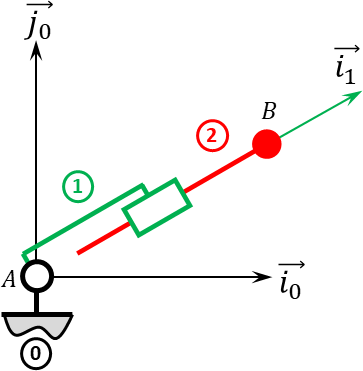
\includegraphics[width=\linewidth]{05_RT_01}
\end{center}
\fi

\question{Tracer le graphe des liaisons.}
\ifprof
\begin{center}
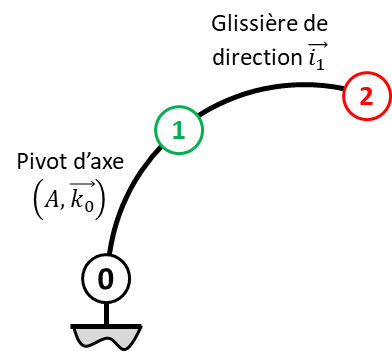
\includegraphics[width=6cm]{05_RT_01_01}
\end{center}
\else
\fi

\question{Retracer le schéma cinématique pour $\theta=\dfrac{\pi}{4}\,\text{rad}$ et $\lambda(t)=\SI{20}{mm}$.}
\ifprof
\else
\fi

\question{Retracer le schéma cinématique pour $\theta=\dfrac{-\pi}{4}\,\text{rad}$ et $\lambda(t)=-\SI{20}{mm}$.}
\ifprof
\else
\fi

\begin{center}
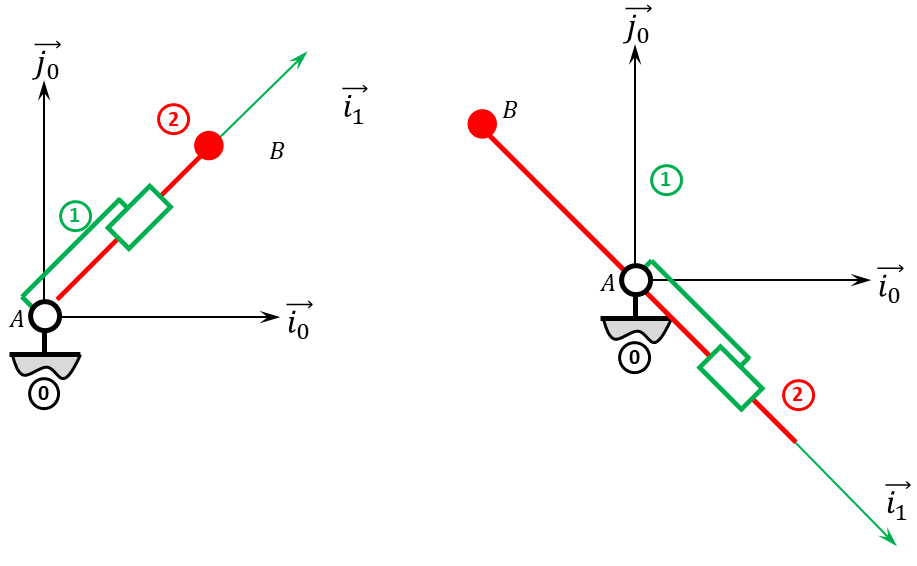
\includegraphics[width=.8\linewidth]{05_RT_01_02}
\end{center}


\ifprof
\else
\begin{flushright}
\footnotesize{Corrigé  voir \ref{B2:12:05}.}
\end{flushright}%
\fi